\chapter{Dashboard Visualisierung} % 5-6 Seiten? 
\label{ch:auswahl}
Im vorherigen Kapitel wurde beleuchtet, wie Nutzerdaten erfasst werden können. Hierfür wurden die relevanten Analysewerte für das Bildungsportal definiert und verschiedene Methoden der Datenerhebung sowie deren DSGVO-konforme Umsetzung erläutert. Um die gesammelten Daten strukturiert und übersichtlich darzustellen und der Professur für Geschichtsdidaktik eine fundierte Grundlage für datenbasierte Erkenntnisse zu bieten, sollen die Analysewerte visuell auf einem Dashboard aufbereitet werden. Dazu werden zunächst technische-funktionale Anforderungen sowie Usability- und Design Anforderungen an das Dashboard definiert. Im Laufe des Kapitels wird zunächst darauf eingegangen, wie die Usability- und Design Anforderungen umgesetzt werden können. Ebenso wird die Struktur sowie der Aufbau des Dashboards bestimmt. Es werden geeignete Visualisierungsmethoden für die Analysewerte definiert und schlussendlich wird Grafana als Visualisierungslösung vorgestellt. Hierbei wird auf das Unterkapitel~\ref{sssec:technfunk} Bezug genommen und beschrieben wie die technisch-funktionalen Anforderungen in Grafana realisiert werden können.

\section{Anforderungen an das Dashboard}
\label{sec:anforderungen}
\subsection{Technisch-funktionale Anforderungen das Dashboard}
\label{sssec:technfunk}
Die technisch-funktionalen Anforderungen sollen bei der Auswahl einer Dashboard Lösung Orientierung geben, welche Funktionen das Tool bereitstellen muss und welche technologischen Rahmenbedingungen erfüllt sein müssen, um eine effiziente Nutzung zusammen mit Matomo zu gewährleisten. Diese Anforderungen sind: 
\begin{itemize}
    \item \textbf{Datenintegration und Aggregation:} Das Dashboard-Tool soll in der Lage sein, die gesammelten Daten von Matomo zu beziehen und zu aggregieren. Außerdem sollen die per Webanalyse-Tool erfassten Daten automatisch aktualisiert werden, entweder in definierten Intervallen oder in Echtzeit.
    \item \textbf{Filtermöglichkeiten:} Es soll die Möglichkeit geboten werden, die erhaltenen Daten zu filtern. Hierbei soll eine Filterung nach Zeitraum und auch eine Filterung nach Unterseite möglich sein, sodass relevante Daten für einzelne Unterseiten analysiert werden könnnen. 
    \item \textbf{Sicherheit und Zugriffskontrolle:} Ebenfalls wie für Matomo, muss auch für Grafana sichergestellt werden, dass nur authentifizierte Benutzer Zugriff auf das Dashboard haben. Somit soll das Dashboard ebenfalls wie Matomo über HTTPS erreichbar gemacht werden. Für die Authentifizierung wird eine ebenfalls eine RBAC benötigt.
\end{itemize}

\subsection{Usability- und Design Anforderungen das Dashboard}
\label{sssec:usability}
Neben technischen Aspekten soll die Benutzerfreundlichkeit gewährleistet sein. Ebenfalls wird auf eine sinnvolle Anordnung und eine geeignete Darstellung für die Analysewerte geachtet. Wichtige Anforderungen sind hierbei:
\begin{itemize}
    \item \textbf{Anordnung der Inhalte:} Die Analysewerte sollen so dargestellt werden, dass verwandte Analysewerte auch im Dashboard nebeneinander zu finden sind.
    \item \textbf{Visualisierung der Inhalte:} Ein einheitliches Farbschema soll die Orientierung erleichtern. Ebenfalls sollen positive und negative Trends einer KPI auf dem ersten Blick zu erkennen sein. Außerdem soll für gleiche Arten von Analysewerten eine konsistente Visualisierungsform genutzt werden, um eine einheitliche Darstellung im Dashboard zu gewährleisten und Verwirrungen zu vermeiden.
    \item \textbf{Responsives Design:} Das Dashboard soll auf verschiedenen Geräten und Bildschirmgrößen benutzerfreundlich dargestellt werden. Die Darstellung soll sich automatisch an unterschiedliche Bildschirmbreiten anpassen, sodass eine Nutzung auf verschiedenen Endgeräten möglich ist.
\end{itemize}

\section{Struktur und Aufbau des Dashboards}
Bei der Gestaltung eines Dashboards ist es sinnvoll, verwandte Daten zu gruppieren, um eine klare Struktur und eine bessere Übersichtlichkeit zu gewährleisten. Besonders bei einer großen Anzahl an Kennzahlen hilft diese Form der Gruppierung dabei, die relevanten Informationen gezielt darzustellen, ohne den Gesamtüberblick zu verlieren. \parencite[Kap.14.3]{Hassler2019}

Ebenso kann, laut Stephen Few, die Möglichkeit zur Navigation zwischen unterschiedlichen Dashboardseiten (engl. Screens) eine sinnvolle Funktion sein. Die Aufteilung der Analysewerte in solche Screens ist allerdings nur dann sinnvoll, wenn dadurch keine Daten fragmentiert werden, welche eigentlich zusammenhängend betrachtet werden sollten. Andernfalls kann eine solche Aufteilung die Effizienz eines Dashboards erheblich einschränken, da zusammengehörige Informationen schwerer in einem sinnvollen Kontext betrachtet werden können. \parencite[Kap.3.1.1]{Few2006}

Auch die Notwendigkeit, innerhalb eines Dashboards vertikal oder horizontal zu scrollen, kann die Übersichtlichkeit und Effizienz beeinträchtigen. Laut Few führt dies dazu, dass Nutzer nicht auf einen Blick alle wichtigen Daten erfassen können und häufig nicht bemerken, dass sich weitere relevante Informationen außerhalb des sichtbaren Bereichs befinden. Elemente, die nicht sofort sichtbar sind, werden oft als weniger wichtig wahrgenommen oder gar übersehen, was die Effektivität eines Dashboards erheblich einschränken kann. \parencite[Kap.3.1.1]{Few2006}

Für das Bildungsportal \textit{evaschiffmann.de} bietet es sich an, die Analysewerte auf einer Haupt-Dashboardseite zusammenzuführen, da diese alle der Analyse des Bildungsportals dienen. Die detaillierte Auswertung einzelner Nutzersitzungen erfordert hingegen deutlich mehr Platz, da je nach Sitzungsdauer und Anzahl der Aktionen eine große Menge an Daten erfasst werden. Um unnötiges Scrollen zu vermeiden und die Übersichtlichkeit zu wahren, wird diese Darstellung daher auf eine separate Dashboard-Seite ausgelagert.

\subsection{Anordnung der Inhalte}
Um nun die Analysewerte auf der Haupt-Dashboardseite so anzuordnen, dass Analysewerte, welche dem selben Kontext dienen nah bei einander angezeigt werden, empfiehlt sich eine Gruppierung nach Untersuchungsthema \parencite[Kap.14.3.1]{Hassler2019}. Diese Untersuchungsthemen sind die in Kapitel~\ref{sec:kpis} erläuterten Dimensionen. Somit werden die Analysewerte auf dem Dashboard so angeordnet wie in Abbildung~\ref{fig:dimensionen} zu erkennen. Metriken zu den Quellen sollen oben links dargestellt werden, Metriken zu den Besuchern oben rechts. Die Inhalte sind unten links zu finden und der Bereich unten rechts soll Aufschluss über das Verhalten der Nutzer geben.

\section{Visualisierung der Inhalte}
\label{sec:Visualisierungsmethoden}
Nachdem die Dashboardstruktur sowie die Anordnung der Inhalte festgelegt wurden, sollen nun geeignete Visualisierungsformen für die Analysewerte bestimmt werden. 
Ein wesentlicher Bestandteil einer effektiven Datenvisualisierung ist eine eindeutige und aussagekräftige Beschriftung. Titel dienen dazu, den Inhalt einer Abbildung prägnant zusammenzufassen und die beabsichtigte Botschaft klar zu vermitteln. Laut Wilke sollte eine Abbildung genau einen Titel besitzen, dieser kann entweder direkt in die Visualisierung integriert werden oder als erstes Element in einer Bildunterschrift angegeben werden. Außerdem sollten die Achsen von Diagrammen immer mit einer entsprechenden Beschriftung versehen sein, welche bei der Zuordnung der Analysewerte hilft. \parencite[Kap.22]{Wilke}

Um Zahlenwerte, welche für bestimmte Kategorien erfasst werden aussagekräftig darzustellen, ist ein Balkendiagramm gut geeignet \parencite[Kap.5]{Wilke}. Hierzu zählt die Metrik \glqq Seitenaufrufe nach Häufigkeit\grqq{}. Dabei stellen die Namen der einzelnen Unterseiten die Kategorien dar, während die zugehörigen Zahlenwerte die Anzahl der Seitenaufrufe repräsentieren.

Die Metriken \glqq Verteilung der Traffic Quellen\grqq{} und \glqq Verteilung der Gerätetypen\grqq{} fallen ebenfalls in diese Kategorie. Da es sich hierbei allerdings um Proportionen handelt und aufgezeigt werden soll, wie die Verteilung über die gesamte Menge ist, ist hierfür ein Kreisdiagramm die bessere Wahl \parencite[Kap.5]{Wilke}.

Da für die Metriken \glqq Ranking der Referer Seiten\grqq{} und dem \glqq Ranking der am häufigsten aufgeklappten Überschriften\grqq{} jeweils Kategorien mit mehreren Zahlenwerten erfasst werden, ist eine tabellarische Darstellung aufgrund der besseren Übersichtlichkeit sinnvoller \parencite{Auditrium}. Für das \glqq Ranking der Referer Seiten\grqq{} soll neben der Anzahl der Besuche über einen bestimmten Referer auch die Anzahl der Beusche erfasst werden, in denen Nutzer nur eine einzige Aktion auf der Website durchgeführt haben. Für das \glqq Ranking der am häufigsten aufgeklappten Überschriften\grqq{} sollen neben dem Titel und der Häufigkeit des Aufklappens auch die Gesamtanzahl aller aufgeklappten Überschriften angezeigt werden.

Einfachen numerischen Metriken, die lediglich aus einem einzelnen quantitativen Wert bestehen, wird keine explizite Visualisierungsform zugewiesen, da sie keine vergleichenden oder relationalen Darstellungen erfordern. Für die Metriken \glqq Anzahl der Besuche\grqq{}, \glqq Anzahl der wiederkehrenden Besucher\grqq{} und \glqq Anzahl der einmaligen Beuscher\grqq{} ist keine zusätzliche Einheit notwendig, da der Zahlenwert selbsterklärend ist. Die \glqq Verweildauer\grqq{} hingegen benötigt eine Einheit um den Wert korrekt interpretieren zu können, weshalb die Zeiteinheit hierbei ebenfalls angegeben werden muss \parencite[Kap.22]{Wilke}. Obwohl es sich bei der Bounce-Rate um eine Verhältnisgröße handelt, soll diese ebenfalls als einfacher Zahlenwert dargestellt werden, um die visuelle Übersichtlichkeit des Dashboards zu wahren und den Anwender nicht mit zu vielen komplexen Visualisierungen zu überfordern. Die Bounce-Rate erhält im Dashboard die Einheit Prozent.

Für die Visualisierung von KPIs wird eine Gauge-Anzeige genutzt. Diese zeigt den numerischen Wert der Zielerreichung an und verwendet eine farbliche Skalierung zur schnellen Interpretation \parencite{GrafanaGauge}. Die Metrik \glqq Anteil der wiederkehrenden Besucher\grqq{} wird ebenfalls über eine Gauge-Anzeige visualisiert.

Für die Visualisierung der individuellen Nutzerinteraktionen innerhalb einer Sitzung konnte keine geeignete bestehende Methode identifiziert werden. Daher soll eine eigene Lösung entwickelt werden, welche auf einem Gantt-Diagramm basiert. Gantt-Diagramme finden typischerweise im Projektmanagement Anwendung und dienen dazu, Aktivitäten über einen bestimmten Zeitraum hinweg darzustellen \parencite{GanttCom}. Für die Analyse individueller Nutzersitzungen wird dieses Konzept adaptiert, um den zeitlichen Verlauf der Nutzeraktionen darzustellen. Die X-Achse repräsentiert die Sitzungsdauer, während die Y-Achse die einzelnen Interaktionen des Nutzers auflistet. Jede Aktion wird durch einen Balken visualisiert, dessen Länge die Dauer der Interaktion widerspiegelt.

All diese Visualisierungen lassen sich mit den Funktionen und Panel-Typen von Grafana umsetzen. Ein Panel besteht aus einer Abfrage an eine Datenquelle und der entsprechenden Visualisierung der Ergebnisse \parencite{GrafanaPanel}. Im folgenden Kapitel wird aufgezeigt, wie Grafana als Dashboard-Tool eingesetzt wird und wie es die technisch-funktionalen Anforderungen an die Dashboard-Lösung erfüllt. Die Konfiguration der Panels erfolgt im Rahmen der Implementierung und wird in Kapitel~\ref{ch:implementierung} erläutert.

\section{Grafana als Dashboard-Tool}
Ebenso wie das Webanalyse-Tool Matomo ist Grafana Open-Source und kann sowohl in einer Cloud-Version als auch in einer On-Premise-Version auf einem eigenen Server betrieben werden. Die Selbsthosting-Variante kann unter anderem auf Linux (Debian/Ubuntu), Windows oder macOS installiert werden. Alternativ lässt sich Grafana auch als Docker-Container über ein offizielles Docker-Image bereitstellen. Grafana verwendet standardmäßig eine SQLite -Datenbank, um das Dashboard, die Datenquellen und die Benutzer der Anwendung zu speichern. Nach der Installation ist Grafana über eine Web-Oberfläche zugänglich, über die Konfigurationen und Dashboards verwaltet werden können. Um diese Web-Oberfläche nutzen zu können, muss JavaScript im Browser aktiviert sein. Unterstützt werden die Browser Chrome, Firefox, Safari und Microsoft Edge. \parencite{GrafanaLabsInstall}

\subsection{Datenintegration und Aggregation}
Die Anbindung von Grafana an Matomo sowie die Aggregation der erfassten Daten kann über diese beiden Varianten erfolgen \parencite{Verteuil2022}, \parencite{MatomoDBConnection}, \parencite{MatomoReportingAPI}, \parencite{MatomoDBSchema}:

\begin{enumerate}
    \item \textbf{Anbindung über die Matomo-Datenbank:}  
    Grafana kann direkt mit der Matomo-Datenbank verbunden werden, indem eine entsprechende Datenquelle eingerichtet wird. Durch SQL-Abfragen auf Datenbanktabellen wie \verb|log_link_visit_action| oder \verb|log_visit| können Rohdaten zu Besuchern, Sitzungen und Interaktionen abgefragt werden. 
    \item \textbf{Anbindung über die Matomo Reporting API:}  
    Alternativ kann Grafana die Matomo Reporting API (Matomo Analytics API) unter anderem als JSON- oder CSV-Datenquelle nutzen. Dadurch können ebenfalls KPIs und standardisierte Matomo-Reports abgerufen werden, ohne direkt auf die Datenbank zuzugreifen. Über die API können Daten ebenfalls für einen bestimmten Zeitbereich aggregiert werden, hierbei ist allerdings die kleinste Einheit ein Tag.
\end{enumerate}

\subsection{Filtermöglichkeiten}
In Grafana ist es möglich, alle auf dem Dashboard oder in den einzelnen Panels angezeigten Daten nach Datum oder Zeitraum zu filtern. Hierfür stellt Grafana einen Zeitbereichsfilter (engl. Time Range) bereit, welcher in die Panels integriert werden kann. Hierbei lassen sich sowohl relative Zeiträume (z. B. die letzten sechs Stunden, der letzte Tag oder die letzte Woche) als auch absolute Zeitangaben mit einem exakt definierten Start- und Enddatum festlegen. Die grafische Oberfläche hierfür, der sogenannte Time Picker, ist in Abbildung~\ref{fig:timerange} dargestellt. Auf der linken Seite können absolute Zeitangaben definiert werden. Auf der rechten Seite gibt es eine Auswahl über relative Zeitangaben, wobei noch zahlreiche Weitere verfügbar sind. Im unteren Bereich des Filters ist es außerdem möglich, die Zeitzone zu konfigurieren. \parencite{GrafanaTimePicker}

\begin{figure}[H]
    \centering
    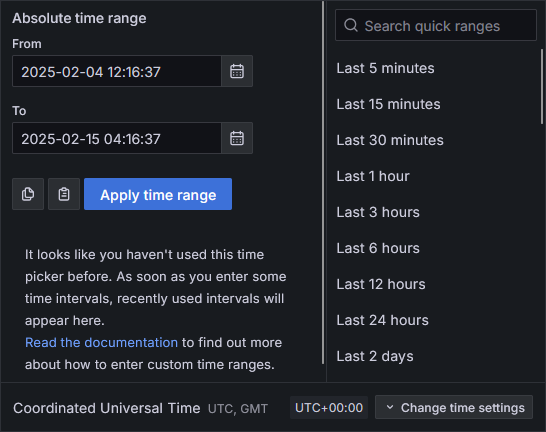
\includegraphics[width=0.6\textwidth, keepaspectratio]{images/timerange.png}
    \caption{Grafana Time Picker}
    \label{fig:timerange}
\end{figure}

Neben der Filterung nach Zeiträumen ermöglicht Grafana die Definition von Variablen, die in den Einstellungen erstellt und je nach Konfiguration auf dem Dashboard angezeigt werden. Diese Variablen dienen als Platzhalter in SQL-Queries oder API-Abfragen. Wählt der Nutzer einen Variablenwert aus, werden alle Panels, die diese Variable enthalten, dynamisch angepasst und zeigen die entsprechend gefilterten Daten an. \parencite{GrafanaLabsVariables}

\subsection{Sicherheit und Zugriffskontrolle}
Um den Zugriff auf das Dashboard zu schützen, stellt Grafana standardmäßig eine integrierte Authentifizierungsfunktion bereit. Bei der ersten Anmeldung wird ein vordefiniertes Admin-Konto mit dem Benutzernamen \verb|admin| und einem Standardpasswort eingerichtet. Aus Sicherheitsgründen sollte dieses Passwort unmittelbar nach dem ersten Login geändert werden. Außerdem liefert Grafana ein rollenbasiertes Zugriffssystem. In der Open Source Version stehen die drei vordefinierten Rollen Viewer, Editor und Admin zur Verfügung. Viewer können Dashboards nur anzeigen, während Editoren zusätzlich Dashboards bearbeiten und neue Panels erstellen dürfen. Administratoren haben vollständigen Zugriff auf alle Konfigurationen innerhalb der Grafana-Instanz. Eine erweiterte rollenbasierte Zugriffskontrolle, die eine feingranulare Berechtigungsverwaltung für Benutzergruppen und API-Zugriffe ermöglicht, ist nur in Grafana Enterprise und Grafana Cloud verfügbar. \parencite{GrafanaRBAC}

Für eine verschlüsselte Verbindung über HTTPS muss in Grafana nichts weiter konfiguriert werden, da hierfür ein Reverse Proxy für die Weiterleitung an Grafana verwendet wird.

\section{Responsive Design}
\label{sec:responsive-design}
Grafana verwendet ein Grid-Layout für die Anordnung der Panels. Diese können auf der Nutzeroberfläche durch den Administrator beliebig in diesem Gitter verschoben werden. Ebenfalls wird standardmäßig der Wert \verb|auto| für die Breite (engl. width) der Panels gesetzt, sodass sich diese automatisch an die Bildschirmgröße des Nutzers anpasst.